\documentclass[11pt, oneside]{article} 
\usepackage{geometry}
\geometry{letterpaper} 
\usepackage{graphicx}
	
\usepackage{amssymb}
\usepackage{amsmath}
\usepackage{parskip}
\usepackage{color}
\usepackage{hyperref}

\graphicspath{{figures/}
                      {/Users/telliott/Desktop/figures/}
                      {/Users/telliott/Dropbox/Github-math/figures/}}
% \begin{center} \includegraphics [scale=0.4] {gauss3.png} \end{center}

\title{Broken Chord}
\date{}

\begin{document}
\maketitle
\Large

%[my-super-duper-separator]

The theorem of the ``broken chord'' is ascribed to Archimedes, although his original work --- the \emph{Book of Circles} --- has been lost.  It was analyzed in proofs collected by the Arabic mathematician Al Biruni in his \emph{Book on the Derivation of Chords in a Circle}.  The theorem was not simply of academic interest, but related to the construction of tables of chords in the \emph{Almagest} by Pappus.

\begin{center} 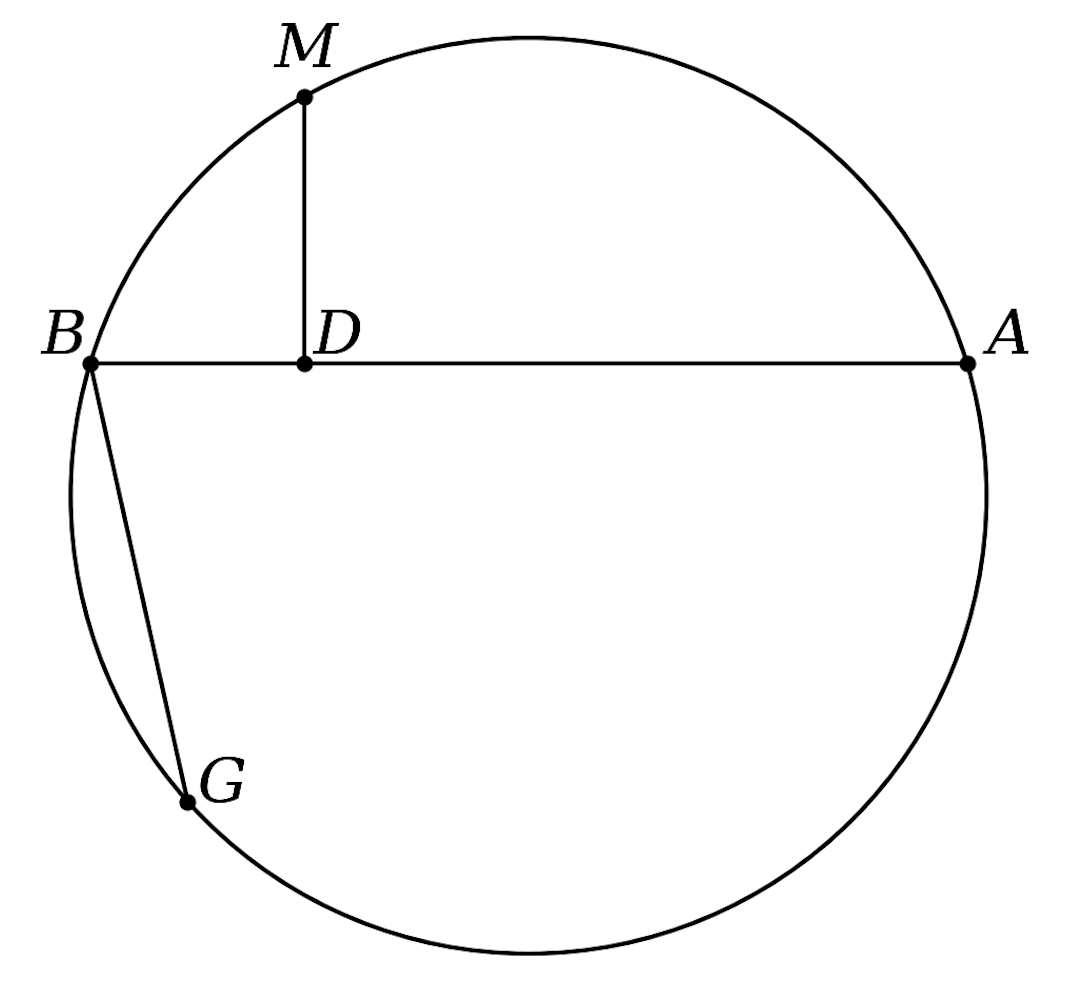
\includegraphics [scale=0.30] {bc00.png} \end{center}
Let $A$ and $G$ be any two points on a circle, and let $M$ be equidistant from both, so that arc $AM$ is equal to arc $GM$.  It does not matter whether $AMG$ is a major or minor arc.

Let $B$ be another point on the circle, lying between $G$ and $M$.  Drop the perpendicular from $M$ to $D$ on $BC$.  The claim of the theorem is that $GB + BD = AD$.

Here we focus first on what are believed to be Archimedes' three proofs, and then continue with several more.  A major motivation is that I have written a library in Python to draw planar geometrical figures.  The advantage is that it is easier to keep a series of figures consistent with each other.

\begin{center} 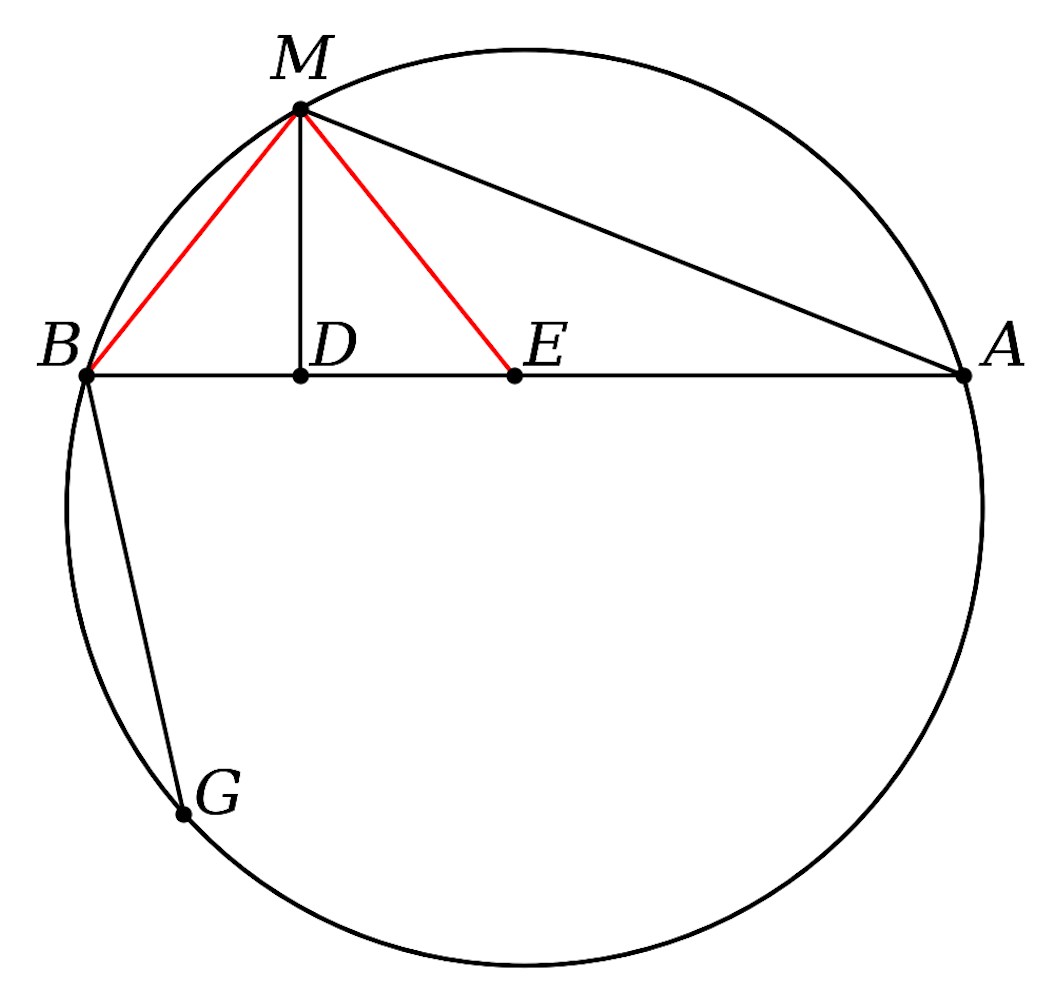
\includegraphics [scale=0.30] {bc0.png} \end{center}

Starting from the figure above, we can, in addition, find point $E \mid BD = ED$.  ($\ \mid \ $ means ``such that'').  We draw $MB$ and $ME$.  $\triangle MBD \cong \triangle MED$ by SAS, so $\triangle MBE$ is isosceles, with $MB = ME$.  This triangle is used for several proofs.

\newpage

\subsection*{first proof}
\begin{center} 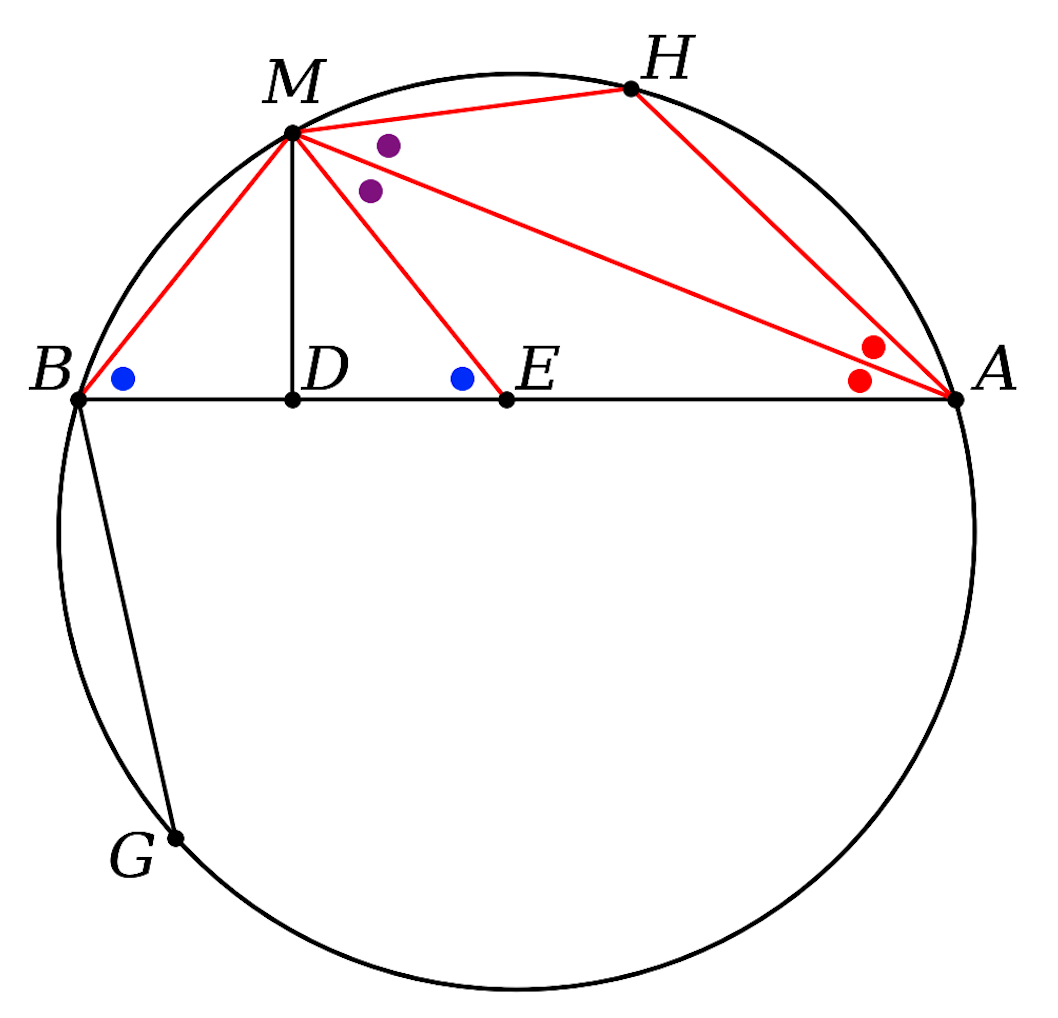
\includegraphics [scale=0.40] {bc1.png} \end{center}

As before, find $E$.  The blue dots indicate equal base angles for an isosceles triangle.

Now find $H \mid MB = MH$.  The red dots indicate angles equal by the well-known corollary of the inscribed angle theorem.

$\angle MBE$ is equal to the sum of red and $\angle HMA$ by the inscribed angle theorem.  

$\angle BEM$ (equal to $\angle MBE$) is equal to red plus $\angle AME$ by the external angle theorem.  

It follows that $\angle HMA = \angle EMA$.  Hence the purple dots.

So $\triangle HMA \cong \triangle EMA$, by ASA.

Then $AE = AH$.  

\begin{center} 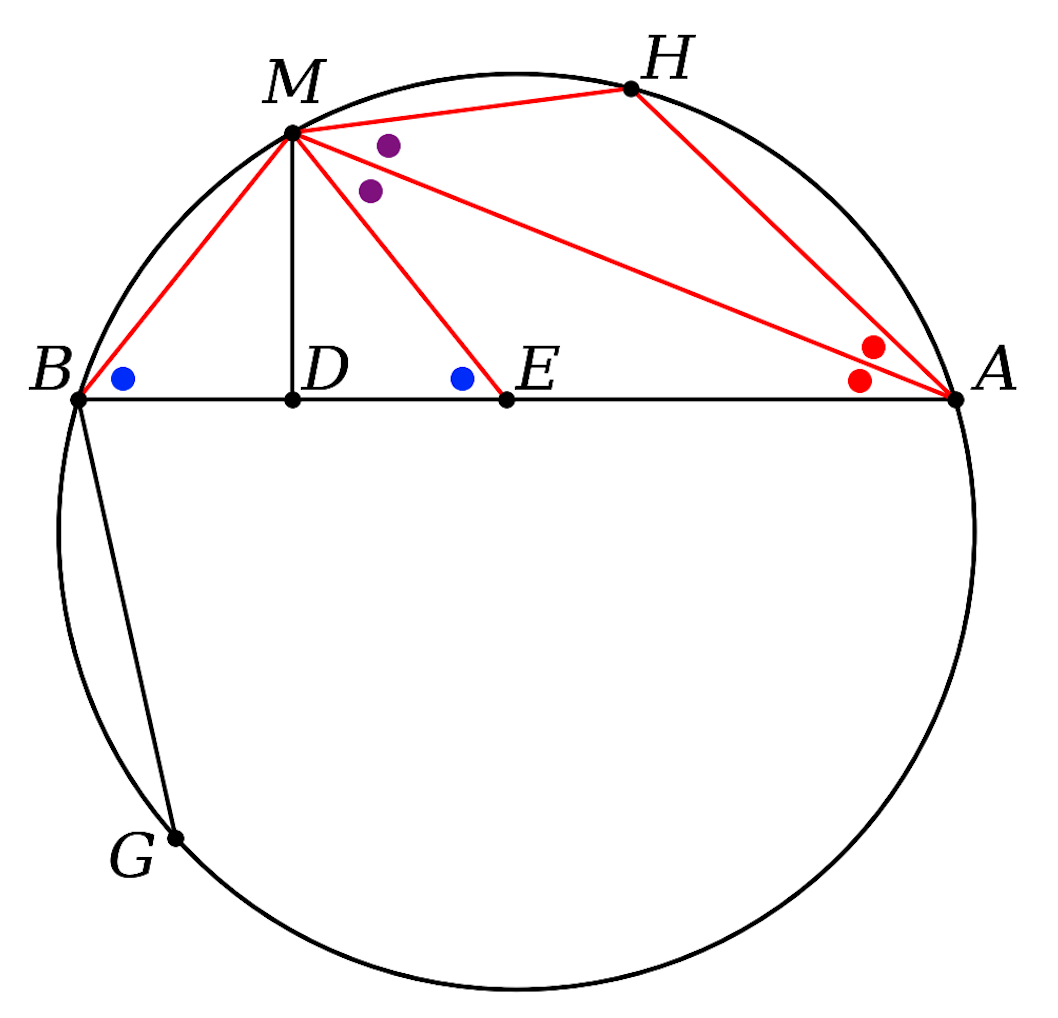
\includegraphics [scale=0.40] {bc1.png} \end{center}

Subtract $MB = MH$ from $GM = AM$, leaving $AH = GB$.  Then
\[ GB = AE \]
Adding equals
\[ GB + BD = AE + ED = AD \]
$\square$

\subsection*{second proof}

\begin{center} 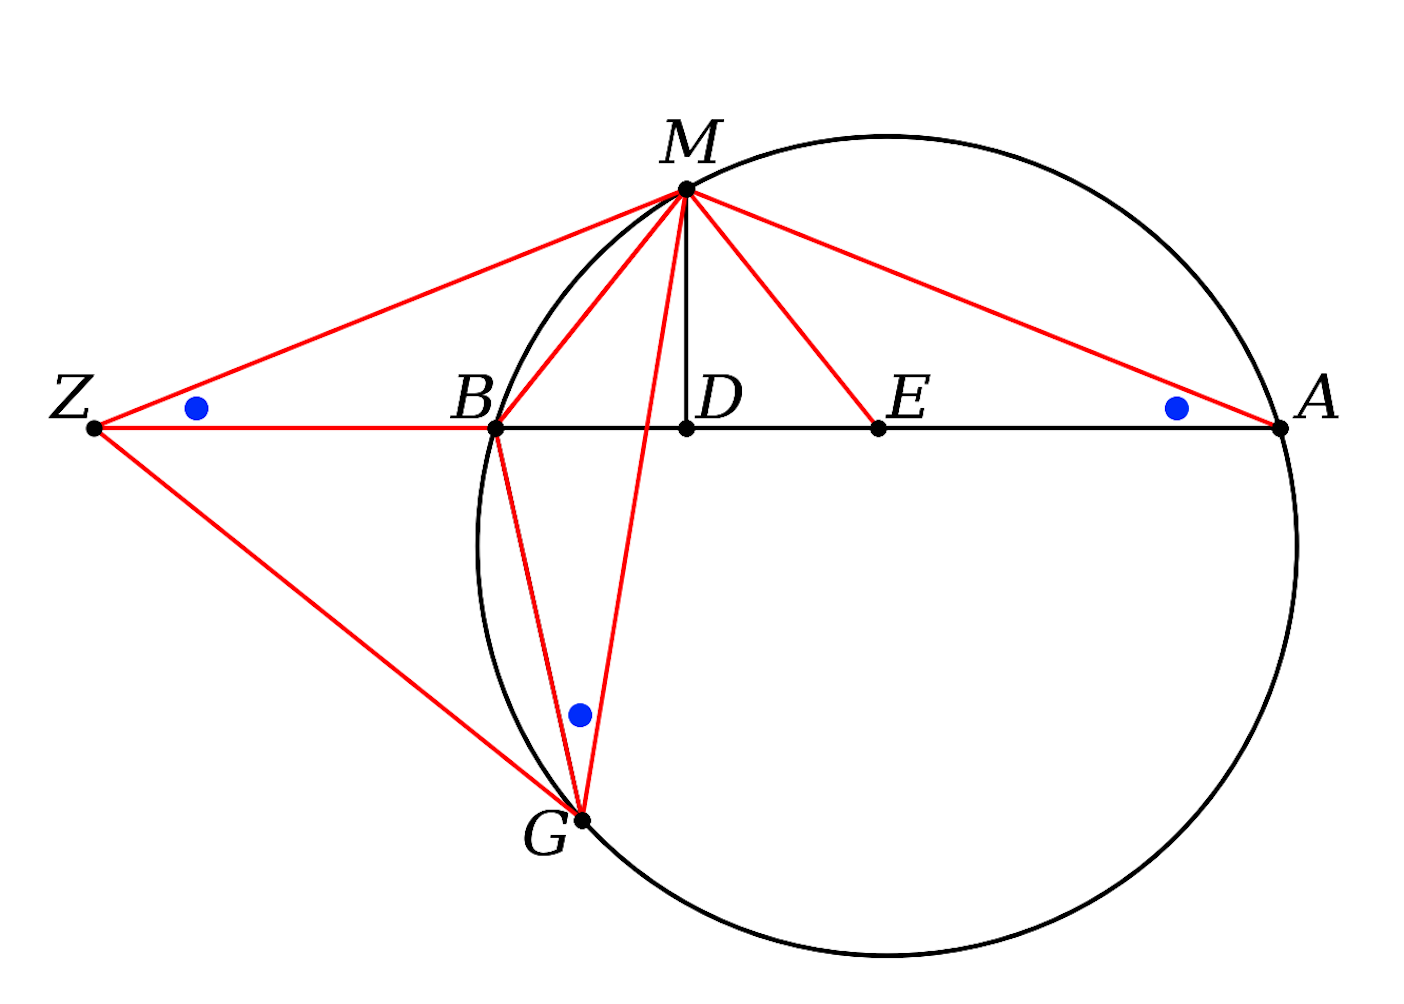
\includegraphics [scale=0.40] {bc2.png} \end{center}

Extend $AB$ to $Z \mid MZ = MA$.

Then $\triangle MZA$ is isosceles with $DZ = DA$ and equal base angles as blue dots.  Draw $GZ$, $GB$ and $GM$.

$\angle BGM = \angle MAB$ by the corollary of the inscribed angle theorem and then $\angle BGM = MZD$ because of the isosceles triangle.

Since $MG = MA = MZ$, $\triangle MZG$ is isosceles, and the whole $\angle Z$ is equal to the whole $\angle G$.

Subtracting the blue dots, $\triangle BZG$ is also isosceles.

It follows that 
\[ ZD = AD \]
\[ ZB + BD = AD \]
\[ GB + BD = AD \]
$\square$

\subsection*{proof 3}

\begin{center} 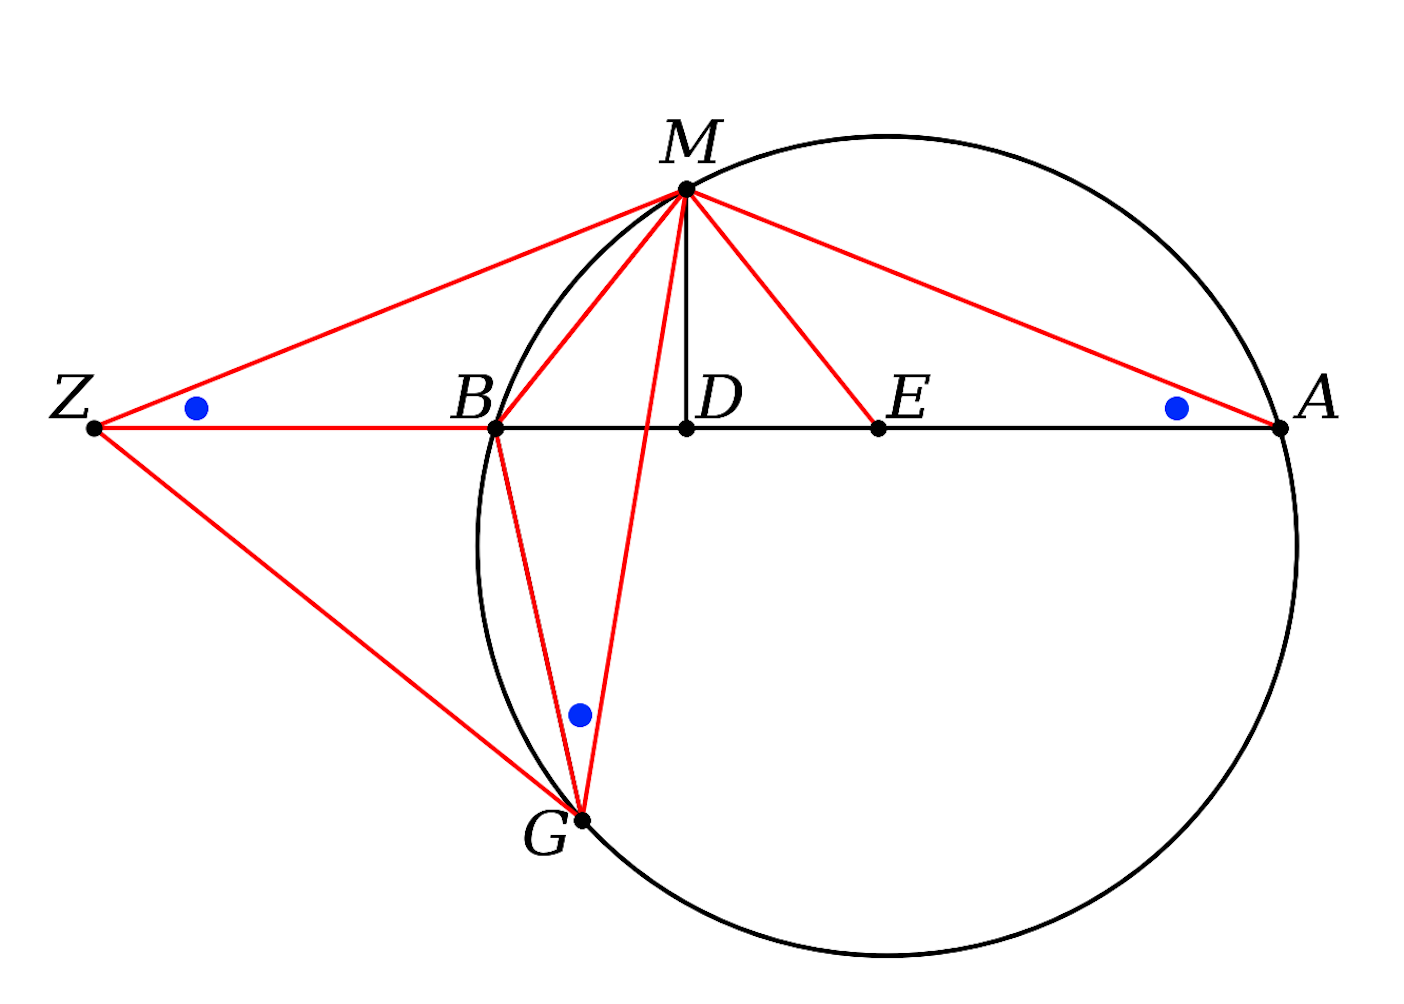
\includegraphics [scale=0.40] {bc2.png} \end{center}

We use the same diagram as in the previous proof.  We will show that $\triangle MBZ \cong \triangle MBG$.

Our construction gives $MA = MZ = MG$ and side $MB$ is shared so in comparing $\triangle MBZ$ and $\triangle MBG$ we have SSA (side-side-angle).

As every student knows, this is not a sufficient criterion for congruence.  However, once it is satisfied, if the two triangles are both acute, or both obtuse, \emph{then they are congruent}.

$\angle ZBM$ is external to $\triangle MBD$ so it is equal to a right angle plus something more.  Therefore $\angle ZBM$ is obtuse.

$\angle MBG$ corresponds to the supplement of arc $MG$.  But $MG = MA$ and together they are less than the whole circle.  It follows that $\angle MBG$ is also obtuse.

So then $\triangle ZBM \cong \triangle MBG$, which gives $ZB = GB$.

By construction
\[ ZB + BD = AD \]
\[ GB + BD = AD \]
$\square$

\subsection*{proof 4}

\begin{center} 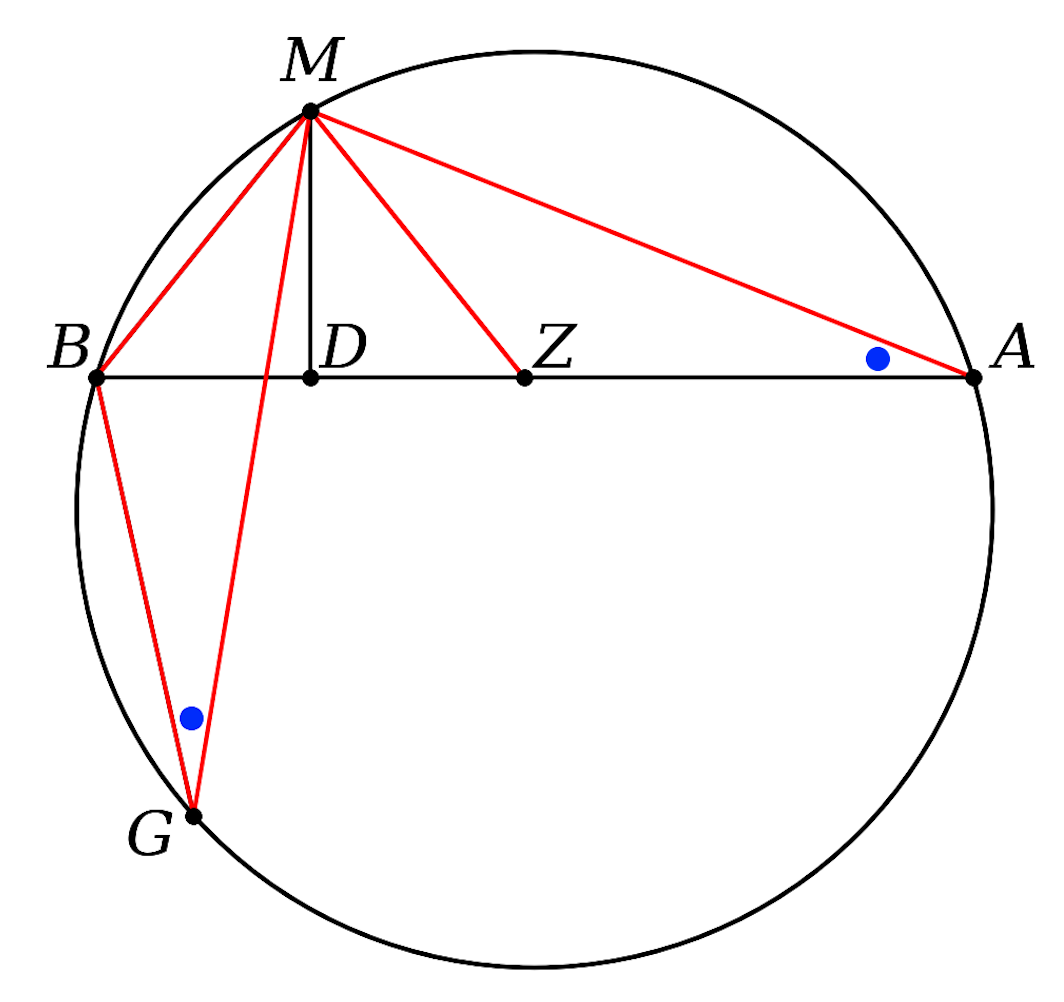
\includegraphics [scale=0.40] {bc3.png} \end{center}

Find $Z \mid AZ = BG$.

We use the point $E$ of the isosceles triangle, but obtain it indirectly, since it turns out that $Z$ and $E$ are the \emph{same point}.

Given the equal angles marked with blue dots (by the corollary of the inscribed angle theorem), we have $AM = GM$ and $AZ = GB$ and the angle in between, so $\triangle BGM \cong \triangle ZAM$ by SAS.

It follows that $MZ = MB$.  (i.e. $Z$ is the same point as $E$).  The proof follows easily in the same way as before.

$\square$

\subsection*{proof 5}

\begin{center} 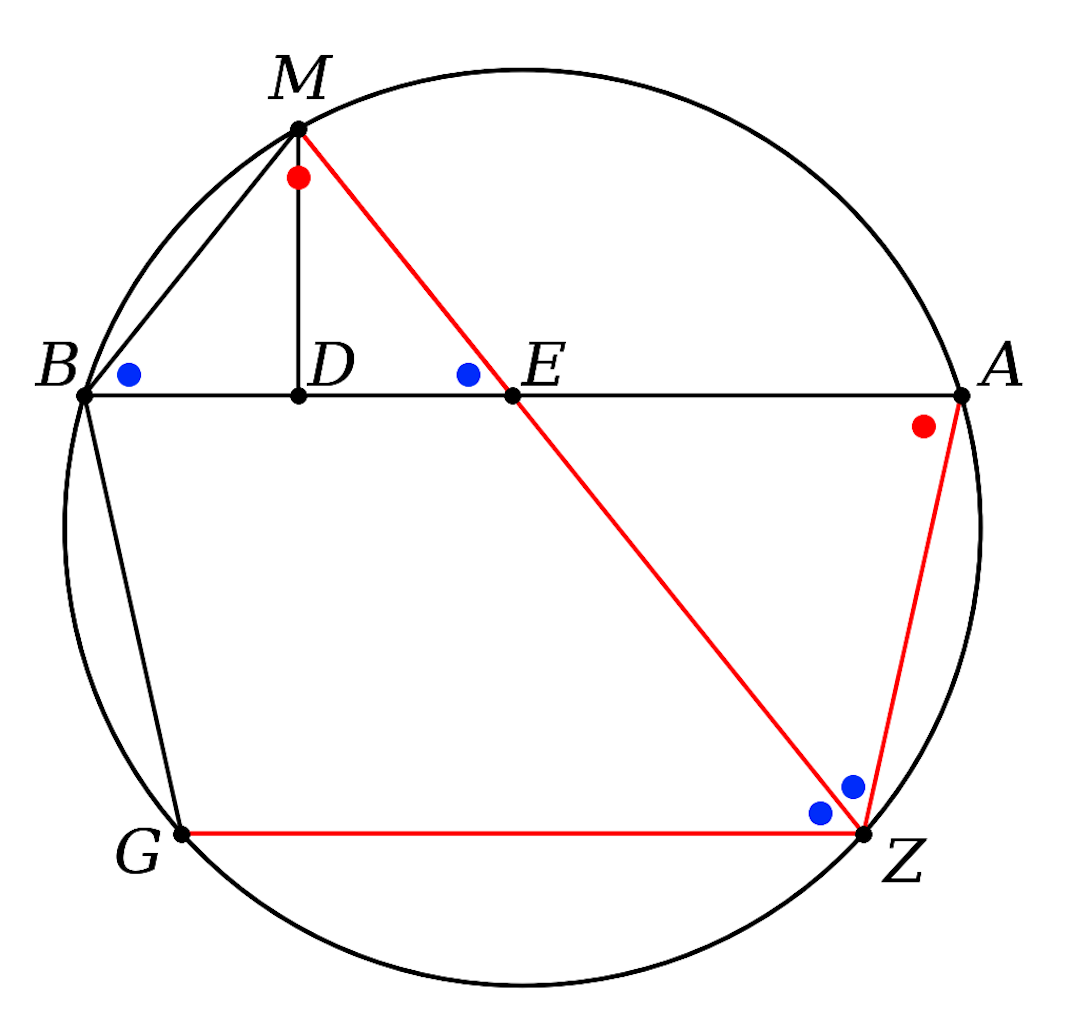
\includegraphics [scale=0.40] {bc5.png} \end{center}

Find $E$ as part of the isosceles $\triangle MBE$ as before and then extend $MB$ to meet the circle at $Z$.  $\angle GZA$ is bisected, since both halves cut equal arcs, and this is the same arc cut by $\angle MBE$.

We also have vertical angles at $E$ ($\angle AEZ$ is not yet marked).

It follows that $\triangle AEZ$ is isosceles, with $AE = AZ$.  The whole angle at $M$ is equal to $\angle A$ because they cut equal arcs, and also by sum of angles.

So then it also follows that $AB \parallel ZG$.  Parallel chords in a circle cut equal arcs.  (We leave this to the reader).  Thus
\[ GB = AZ = AE \]
Adding equals
\[ GB + BD = AE + ED = AD \]

$\square$

However, this proof is incomplete, since for a given arrangement of $G$, $A$ and $D$, depending on the placement of $B$, one can draw $H$ in three different ways --- coincident with $G$, or lying on either side of it.

\begin{center} 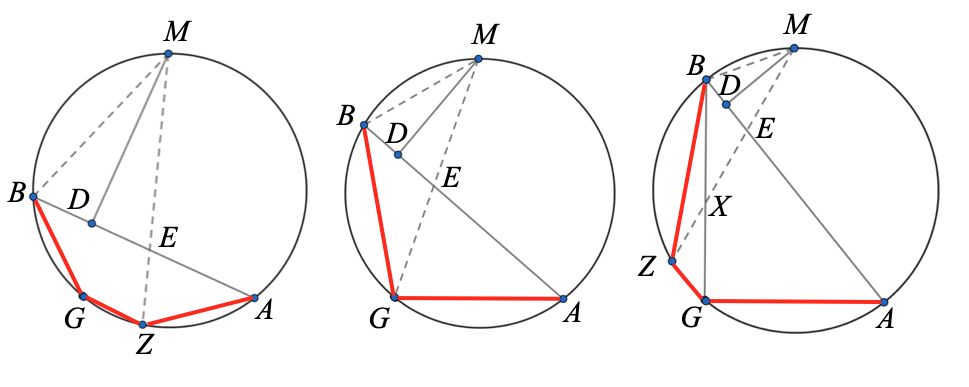
\includegraphics [scale=0.40] {bc5d.png} \end{center}

The left panel is similar to our original diagram.  Some of the points are labeled differently.  But the important thing is that $A$ and $G$ are closer together, and $B$ is fairly close to $M$.

As a result, in the right panel, it appears that $GH \parallel AB$.  Can the proof be rescued?  We redraw the standard figure with $Z$ CW from $G$.

\begin{center} 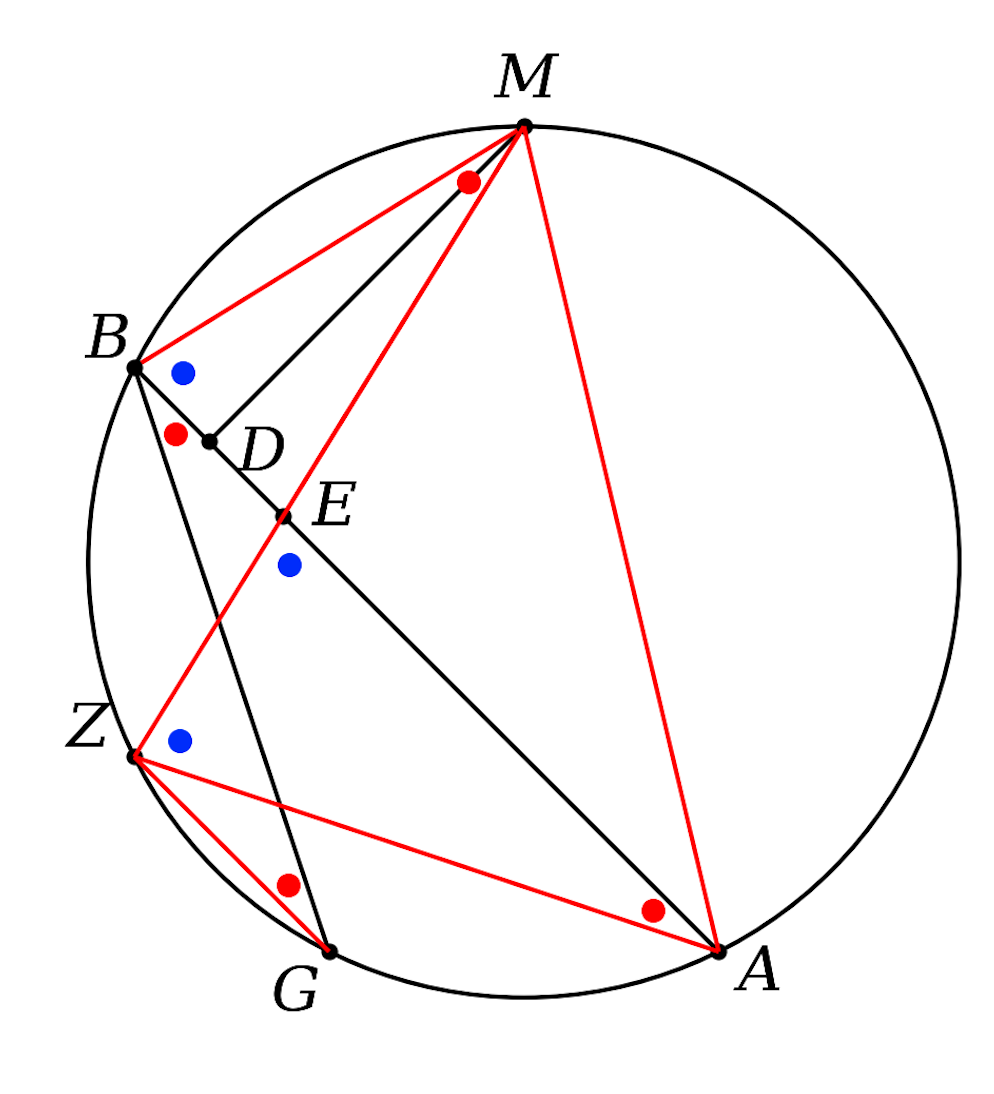
\includegraphics [scale=0.40] {bc5b.png} \end{center}

Three of the angles marked with red dots are on arc $BZ$.  

The fourth one, $\angle ABG$, cuts arc $AG$, which means that it is supplementary to two copies of $\angle MBE$ each cutting the arc $AM$.  So they are all equal.

The angles marked blue either cut the same arc or are equal by vertical angles and the isosceles $\triangle MBE$.

It follows that $GZ \parallel AB$ so $BZ = AG$ and thus $\triangle ZGB \cong \triangle GZA$.

Then $AZ = GB$ and since $\triangle AEZ$ is isosceles
\[ AZ = AE = GB \]

Adding equals
\[ AE + DE = GB + BD \]
\[ AD = GB + BD \]

$\square$ 

The \textbf{third case} is where the extension of $DZ$ terminates exactly on point $G$.  $Z$ coincides with $G$.

\begin{center} 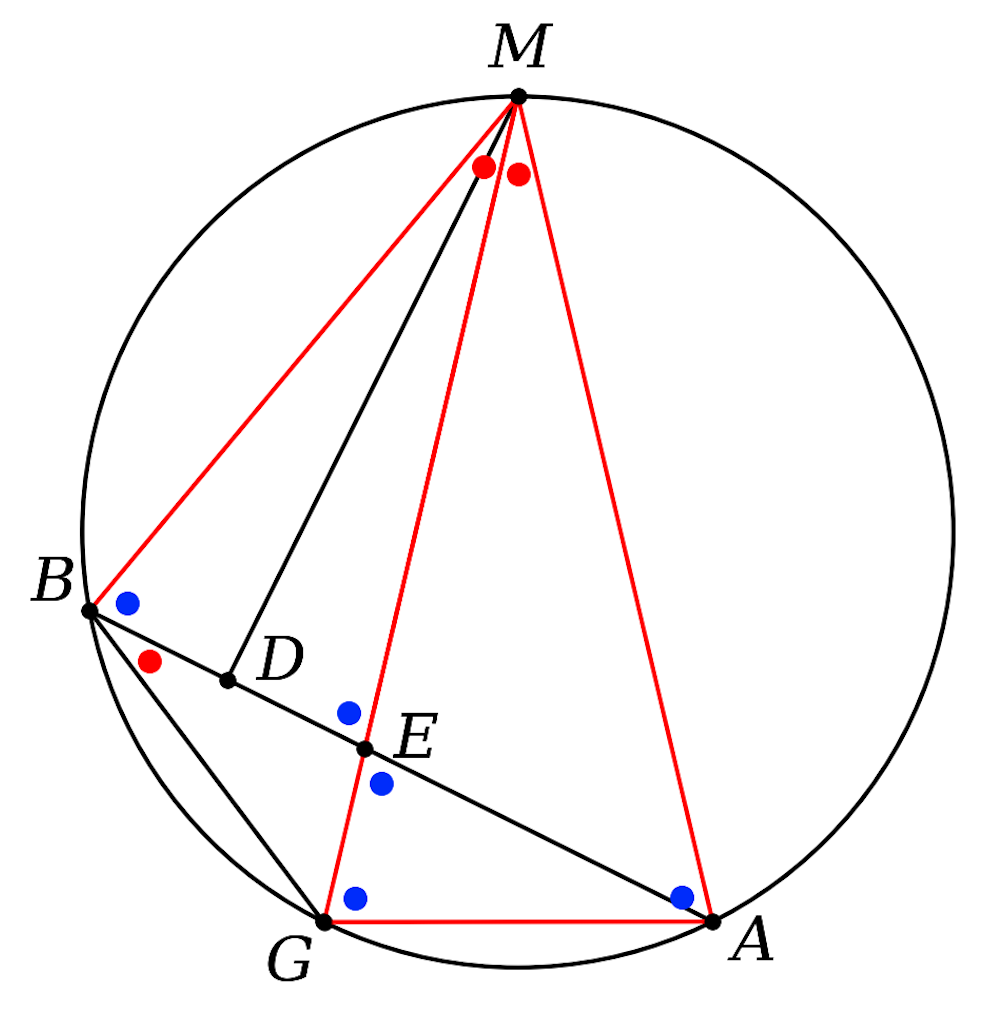
\includegraphics [scale=0.40] {bc5c.png} \end{center}

A nice proof is to complete $\triangle MGA$.  Since $GM = AM$, the triangle is isosceles, with equal base angles cutting arcs equal to that of $\angle MBE$.  It follows that $MG$ bisects $\angle AMB$.

So
\[ \angle EMB = \angle EMA = \angle EBG \]
Then $\triangle ABG$ is isosceles, with $BG = AG$ and $\triangle AEG$ is isosceles as well.  It follows that
\[ AG = AE = BG \]
Adding equals
\[ BG + BD = AE + ED = AD \]

$\square$

\newpage

\subsection*{proof 6}

\begin{center} 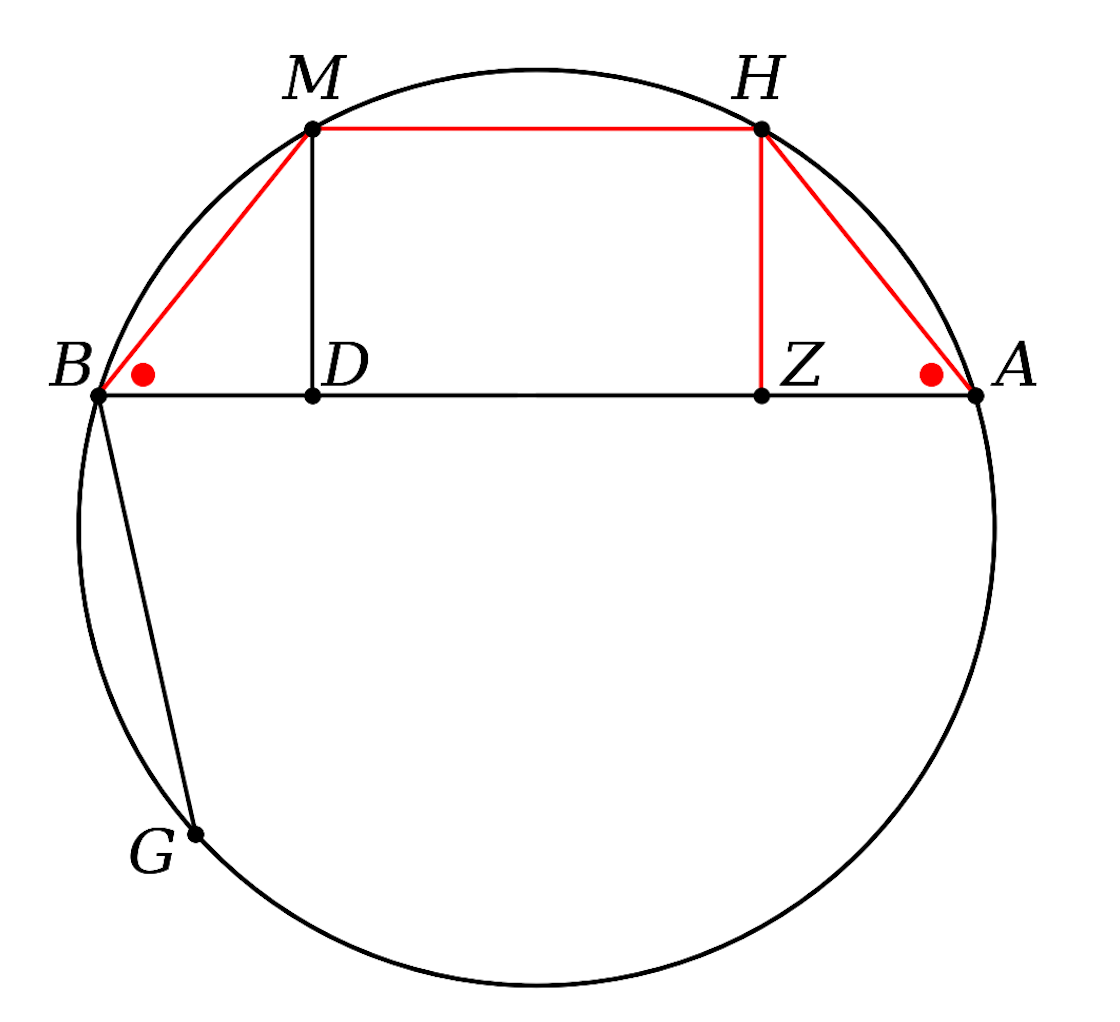
\includegraphics [scale=0.40] {bc6.png} \end{center}

Draw the rectangle $MHZD$, by drawing $MH \perp MD$ to meet the circle at $H$, and then $HZ \parallel MD$.

It is easy to show that the red dotted angles are equal (draw $AM$ and $BH$), and then we have two congruent right triangles in $\triangle MBD$ and $\triangle HAZ$.

So $BD = AZ$.

Given arc $MG = MA$, and $MB = AH$, so find $MH = BG$.

\[ GB + BD = MH + AZ = DZ + AZ = AD \]

$\square$

\newpage

\subsection*{proof 7}

\begin{center} 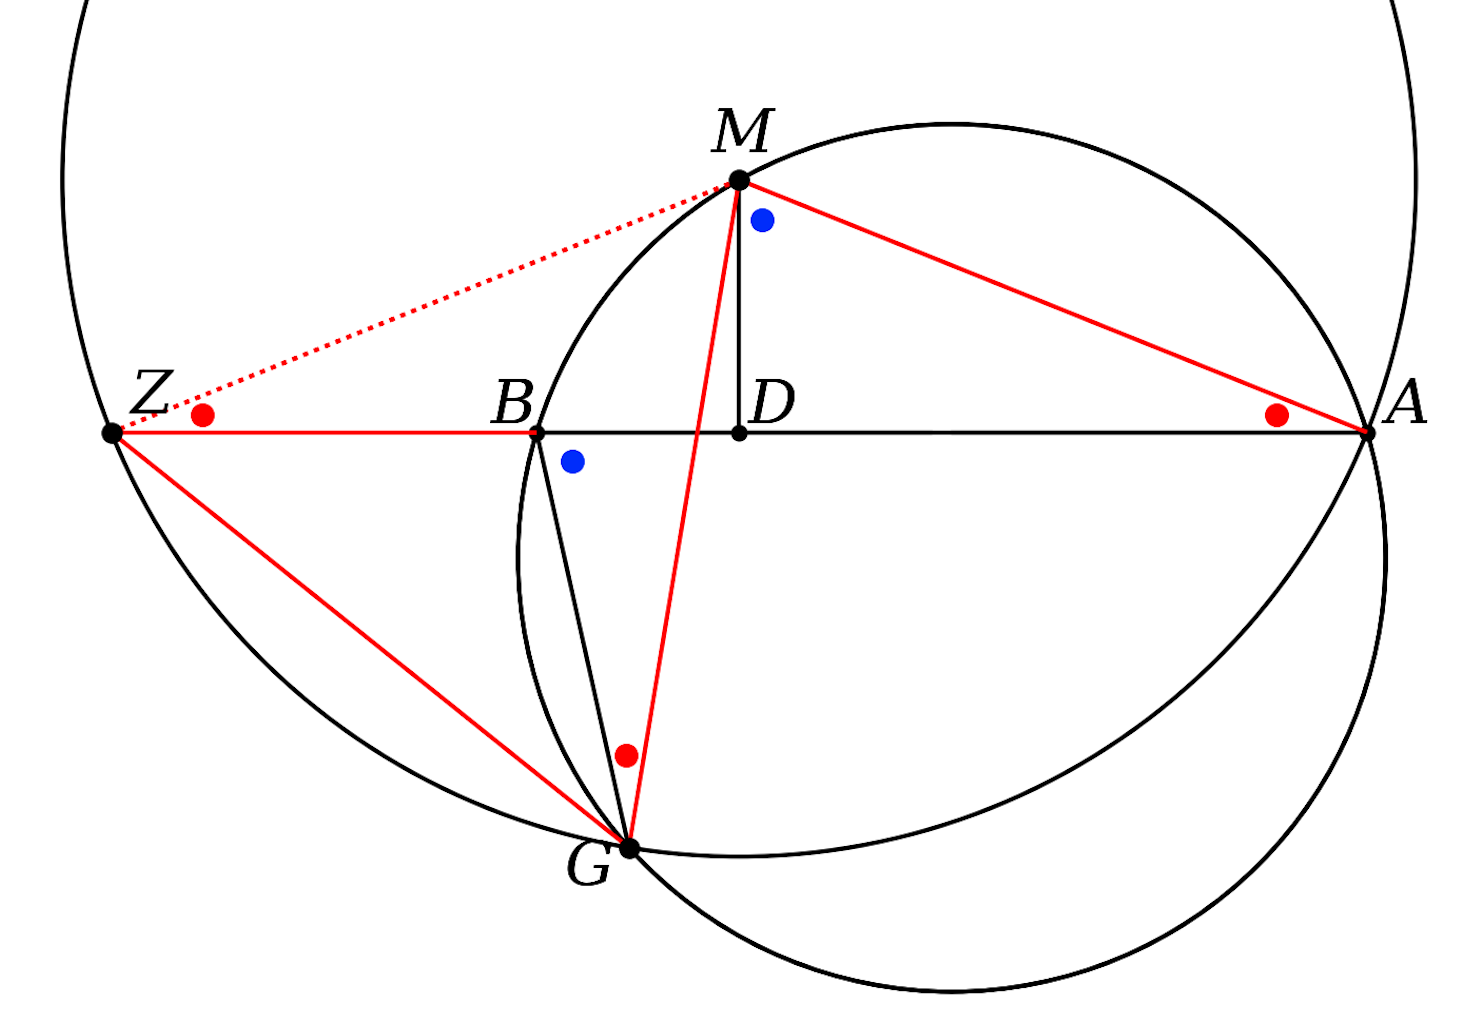
\includegraphics [scale=0.40] {bc7.png} \end{center}

Draw the circle on center $M$ with radius $MA = MG$.  Extend $AB$ to meet the circle at $Z$.

$\angle BGM =  \angle  A$ by inscribed angles.

Since $MZ = MA$, $\triangle MZA$ is isosceles, with $\angle MZD =  \angle A$.  This explains the angles marked with red dots.

The angles marked with blue dots are equal by inscribed angles.

Since $MZ = MG$, $\triangle MZG$ is isosceles, with $\angle MZG =  \angle MGZ$.  $\angle BZG =  \angle BGZ$ by subtraction.

Hence, $\triangle ZBG$ is isosceles and $BG = BZ$.

Given $MD \perp AB$.  $AZ$ is a chord of the circle and $MD$ is perpendicular through the circle center, so $AZ$ is bisected at $D$.

$AD = ZD = ZB + BD = GB + BD$

$\square$

\subsection*{proof 8}

\begin{center} 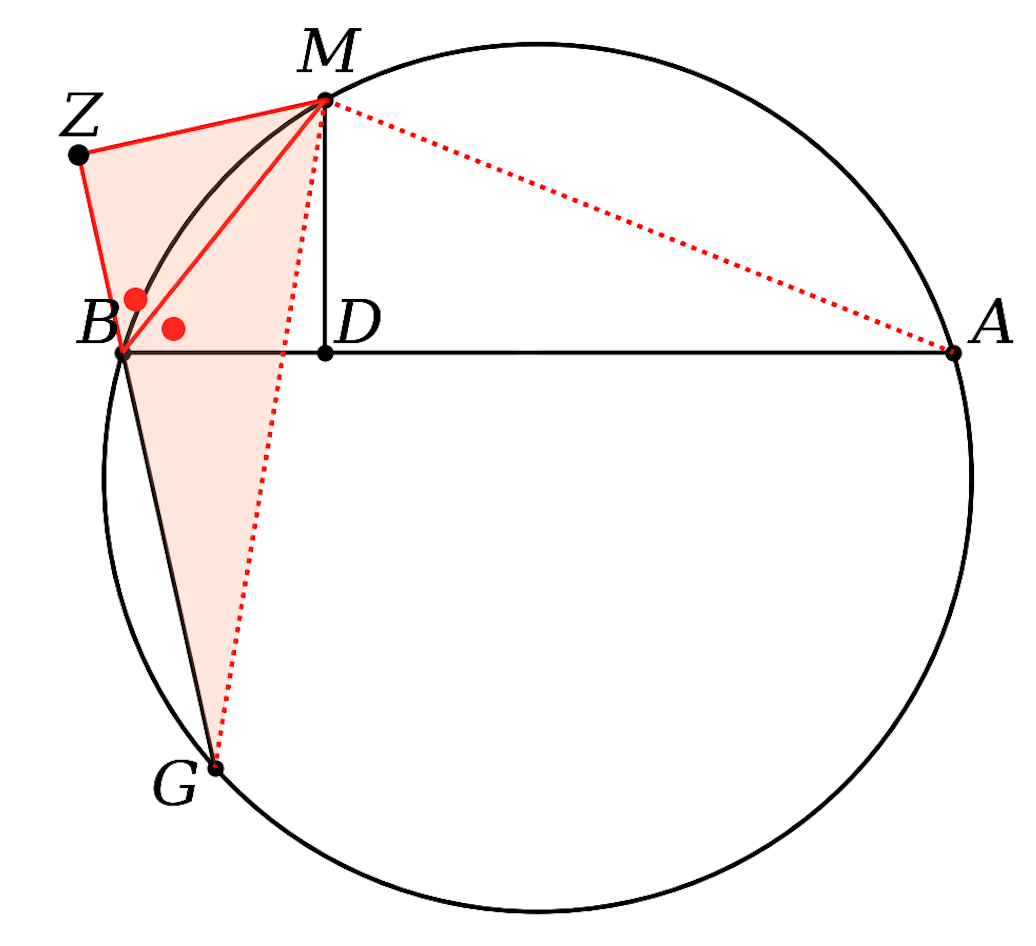
\includegraphics [scale=0.40] {bc8.png} \end{center}

Extend $GB$ to $Z \mid MZ \perp GZ$.

$\angle MBG$ is supplementary to $\angle MBZ$.  $\angle MBG$ lies on arc $MAG$.  Hence, $\angle MBZ$ corresponds to arc $MG$.

But $MG = $MA and $\angle MBD$ lies on arc $MA$, hence the red dots for equal angles.

$\triangle MBZ$ and $\triangle MBD$ are right triangles, sharing a second angle and one side, so they are congruent by ASA.  $BZ = BD$.

Now consider $\triangle MZG$ and $\triangle MDA$.  Both are right and also $\angle A = \angle G$.  Further, $MG = MA$.  So they are congruent with 
\[ AD = GZ = GB + BZ = GB + BD \]

$\square$

\subsection*{proof 9}

\begin{center} 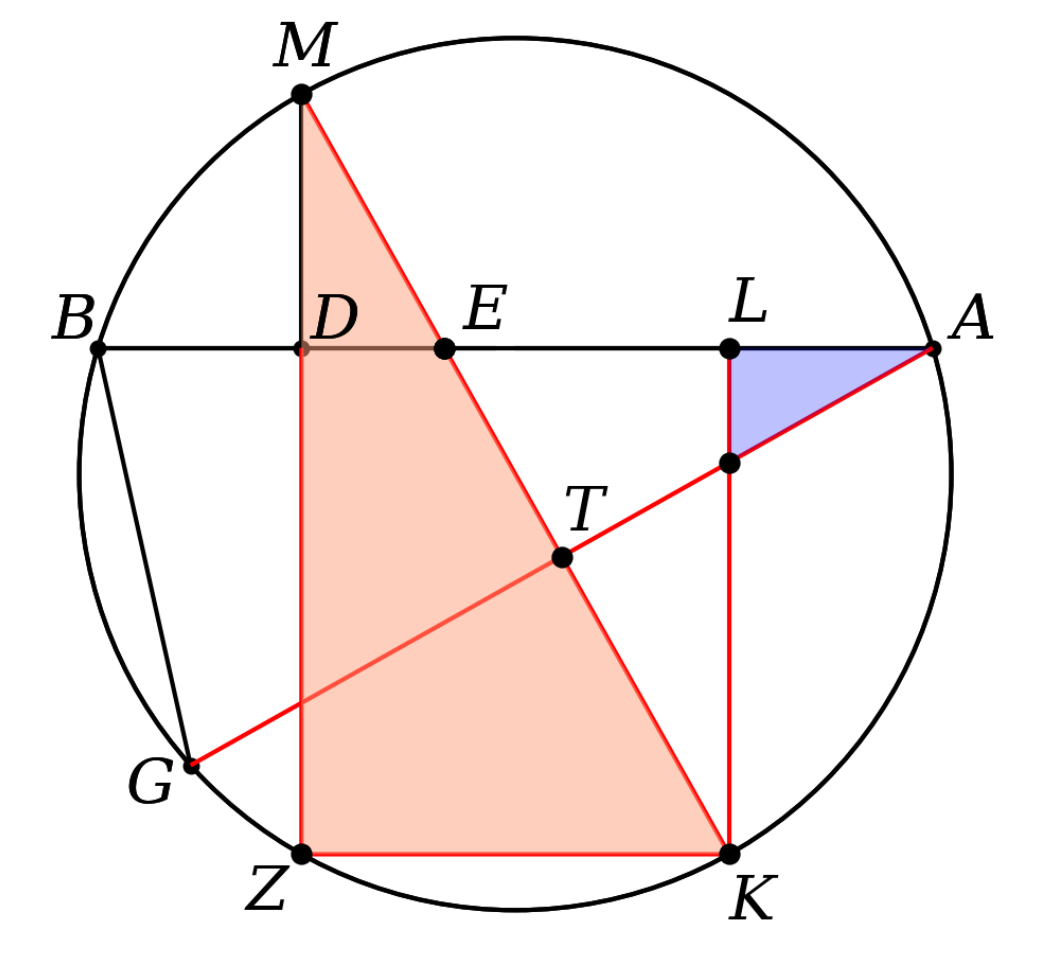
\includegraphics [scale=0.40] {bc9.png} \end{center}

Extend $MD$ to the circle at $Z$.  Draw $MK$ as a diameter of the circle.

Draw $AG$.  Find where $MK$ crosses $AG$ at $T$.  

Also draw $LK \perp AB$.  So $MZ \parallel LK$.

The angle at $Z$ is right, by Thales circle theorem, and $ZK \parallel AB$.  

Thus $DLKZ$ is a rectangle with $ZK = DL$.

$MK$ traverses parallel lines so $\angle M = \angle LKM$

$\triangle LEK$ is similar to the blue triangle, hence $\angle A = \angle LKM = < M$

But $AL = BD$ because $DLKZ$ is a rectangle in a circle.  It follows that

As arcs of equal angles, $BG = ZK = DL$.

\[ BG + BD = DL + AL = AD \]

$\square$

\end{document}